%
%  Fountain Music README
%
\documentclass[11pt]{article}

% Use utf-8 encoding for foreign characters
\usepackage[utf8]{inputenc}

% Setup for fullpage use
\usepackage{fullpage}

% This is now the recommended way for checking for PDFLaTeX:
\usepackage{ifpdf}

\ifpdf
\usepackage[pdftex]{graphicx}
\usepackage[pdftex]{hyperref}
\else
\usepackage{graphicx}
\usepackage{hyperref}
\fi

\title{Fountain Music 2.25}
\author{Brian Moore}

\begin{document}

\ifpdf
\DeclareGraphicsExtensions{.pdf, .jpg, .tif}
\else
\DeclareGraphicsExtensions{.eps, .jpg}
\fi

\maketitle
\begin{center}
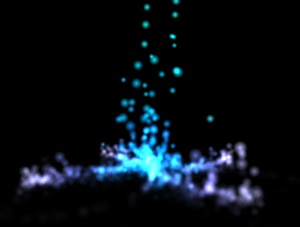
\includegraphics{fmimage.jpg}
\end{center}

Fountain Music is an iTunes visualization which animates a fountain of particles exploding to the music.

\section*{Installation}
To install Fountain Music, just drag the file ``Fountain Music.bundle'' onto the installer icon.  The installer will tell you if installation was successful and where the plugin was placed.  If installation fails, do not fret, you can still attempt a manual install. (see ``Manual Install/Uninstall'')

\section*{Use}
To activate Fountain Music, simply select it in the Visualizer menu and turn on the visualizer in the same menu.  You can make it enter or exit full screen mode by pressing  cmd-F.

Once Fountain Music has been launched, you can make it display the current track info by pressing the letter \verb|i|. The \verb|[ ]| and \verb|\| keys are used for control over the fountain patterns.  Pressing \verb|[| and \verb|]| selects the previous and next patterns, respectively. Pressing \verb|\| stops the pattern from switching on its own.

Just below the pattern controls,\footnote{well, below on QWERTY keyboards, sorry Dvorak-ers} the \verb|;| (semicolon) and \verb|'| (single quote) keys change the color scheme, switching to the next and previous color schemes, respectively.

By pressing the \verb|<| and \verb|>| keys, you can make the particles have fuzzier or sharper edges, respectively.  The \verb|~| key will display the advanced menu, which tells of the keys to press to toggle display of frame rate (\verb|f| key) or number of particles (\verb|p| key).

The \verb|+| and \verb|-| keys make the particles bigger and smaller, respectively. \verb|v| shows the current version.  If you forget any of these controls, there is a menu available by pressing \verb|h|, \verb|?|, or \verb|~|.

To summarize, the key commands are:

\begin{tabular}{c|l}
\verb|h ?| & 	display the help menu                    \\
\verb|+ -| &  	increase or decrease particle size       \\
\verb|[ ] \|&  	previous/next/lock fountain pattern  \\
\verb|; '| &  previous/next color scheme                \\
\verb|< >| &  fuzzier/sharper edges                     \\
\verb|i|   & display track information                  \\
\verb|~|   & display advanced menu                      \\
\verb|p|   & toggle particle count                      \\
\verb|f|   & toggle frame rate display                  \\
\verb|v|   & show version                               
\end{tabular}

Finally, the settings dialog is accessible via the ``Options..." menu item at the end of the View $\rightarrow$ Visualizer menu.  The ``Default" button will return all preferences to their factory values. ``OK" closes the dialog window and keeps all changes you have made. ``Cancel" also closes the window, but it does not save your changes.

\section*{About the Color Schemes}
Beginning with version 2.0, there are a variety of color schemes included with Fountain Music.  These schemes determine what colors particles will be.  Some color schemes change subtly over time, so if you wait for a few seconds the fountain may have an entirely different feel to it. In more detail, the color schemes are:

\begin{description}
\item[Classic]
The original Fountain Music color scheme.  The fountain progresses slowly through the color wheel.
\item[Red, White and Blue]
Did you know that these three colors are the main colors of the flags of Chile, France, Liberia, Malaysia, The Netherlands, Nepal, North Korea, Norway, Iceland, Panama, Puerto Rico, Taiwan, Luxembourg and the UK?\footnote{Source: CIA World Factbook (http://www.cia.gov/cia/publications/factbook/)}  Hmm, wait a second, that list seems a bit short, I definitely forgot a few minor places.  Oh well, email me if you figure it out.
\item[Fire] 
Your music bursts into flames with this color scheme!  Okay, not literally, that would be quite unfortunate, but it does look nice and warm.  Large particles with fuzzy edges are recommended for the full firey effect.
\item[Random]
Particles appear in whatever color they feel like.  In a way, it reminds me of a birthday party, or clowns, or rainbow sprinkles.  Oh no, now I want ice cream, thanks a lot Fountain Music!
\item[Sea]
A blue-greenish color scheme.  The fountain looks vaguely like elegantly flowing water from the deep sea... after it has been thrown into a blender with some seaweed and blue food coloring.
\item[Snow]
A pure white color scheme. Make snow with your music!  Particles look like snowflakes, except for the fact that they're all the same shape unlike their real life versions.
\end{description}

\section*{Manual Install/Uninstall}
To install manually, copy ``Fountain Music.bundle" to the \verb|Library/iTunes/iTunes Plug-ins| folder in your home folder (\verb|/Users/you/|) if you want to keep it all for yourself, or to the aforementioned folder in \verb|/Library/| if you care to share it with other users on your computer.  Create these folders if either does not exist. The next time you start up iTunes, Fountain Music will appear in the ``Visualizer" menu.

To uninstall manually, simply drag ``Fountain Music.bundle" from wherever you put it (see above) to the trash and restart iTunes.

\section*{Source Code}
If you would like the source code for Fountain Music, you can get it under the GPL!  Simply visit \href{www.binaryminded.com}{www.binaryminded.com} and visit Fountain Music in the Software section of the site.

\emph{Binary Minded Software; \href{www.binaryminded.com}{www.binaryminded.com}; bmoore [at] binaryminded [dot] com}

\section*{Version History}
\begin{itemize}
\item June 9, 2008, v.2.25
\begin{itemize}
    \item Slightly refined particle appearance
\end{itemize}
    
\item August 16, 2007, v.2.23
\begin{itemize}
    \item Fixed ``glitchy/broken window" bug
\end{itemize}

\item November 17, 2006, v.2.2
\begin{itemize}
\item Overall stability improvements
\item Released as free software under the GPL
\end{itemize}

\item March 31, 2006, v.2.1
\begin{itemize}
\item Universal binary
\item Full unicode support for track names
\item Control over text size for track info
\end{itemize}

\item December 29, 2005, v.2.0
\begin{itemize}
\item Antialiased text
\item Multiple color schemes
\item Easy installer and uninstaller
\item Gravity control range expanded
\item Minor speed and graphical improvements, as always
\end{itemize}

\item June 18, 2004, v.1.2
\begin{itemize}
\item Controllable gravity
\item Settings dialog, controls gravity, particle size, edges, etc.
\item Saves preferences between relaunches (of iTunes)
\item Continuous FPS calculation
\item Smoother motion at lower frame rates
\item Option to always show track info
\item Some graphical tweaks
\end{itemize}

\item December 30, 2003, v1.15
\begin{itemize}
\item Full resolution in full screen, \verb|r| key rotates resolutions
\item Version display (\verb'v' key)
\end{itemize}

\item December 24, 2003, v1.14
\begin{itemize}
\item Two new modes, Starfish and Flower, bringing the total to 8
\item Speed improvements
\item Four months worth of minor tweaks
\end{itemize}

\item August 24, 2003, v1.12
\begin{itemize}
\item Fixed a bug which caused iTunes to crash when the user rated a song
\item Added control over the particle edge sharpness (\verb'<' and \verb'>' keys)
\item Added FPS and particle counters (\verb'f' and \verb'p' keys, respectively)
\item Added an advanced menu (\verb'~' key)
\item Now remembers settings between uses
\item Many internal improvements and some minor graphical bugs fixed.
\end{itemize}

\item August 21, 2003: v1.11
\begin{itemize}
\item Added control over the modes
\item Speed improved
\item Both audio channels are used
\item Fixed a bug which prevented some from using it
\end{itemize}

\item August 5, 2003: v1.1
\begin{itemize}
\item Changed the fountain around a bit 
\item Much more responsive to the music 
\item Added 6 different fountain modes 
\item Added a menu feature accessible by typing \verb'?' or \verb'h' 
\item The particle size is controllable by \verb'+' and \verb'-' 
\item Other minor improvements and bug fixes 
\end{itemize}

\item June 3, 2003: v1.0
\begin{itemize}
\item Initial release
\end{itemize}
\end{itemize}

\begin{center}
    Copyright \copyright 2005-2008 Binary Minded Software
\end{center}

\end{document}
